\documentclass[11pt,letterpaper]{article}
\usepackage[T1]{fontenc}
\usepackage[scaled]{helvet}
\renewcommand{\familydefault}{\sfdefault}
\usepackage{amsmath,amssymb}
\usepackage[margin=0.8in,bottom=0.9in]{geometry}
\usepackage[most]{tcolorbox}
\usepackage{tikz}
\usetikzlibrary{calc}
\usepackage{enumitem}
\usepackage{array}
\usepackage{needspace}
\usepackage{fancyhdr}
\usepackage{pifont}

% ---- Palette "F. Bright & Playful" ----
\definecolor{fmtitle}{HTML}{3D2C8D}
\definecolor{fmkey}{HTML}{0096C7}
\definecolor{fmwatch}{HTML}{2BB673}
\definecolor{fmturn}{HTML}{F4A100}
\definecolor{fmmistake}{HTML}{EF476F}
\definecolor{fmnotice}{HTML}{9B5DE5}
\definecolor{fmgray}{HTML}{6B6B6B}

\pagestyle{fancy}
\fancyhf{}
\renewcommand{\headrulewidth}{0pt}
\fancyfoot[C]{\footnotesize\color{fmgray}\textcopyright\ 2026 FangMath. All rights reserved.}
\fancyfoot[R]{\footnotesize\color{fmgray}\thepage}
\setlength{\parindent}{0pt}
\setlength{\parskip}{3pt}

\newcommand{\badge}[1]{\colorbox{fmtitle}{\color{white}\bfseries\small\ #1\ }}
\newcommand{\leveltag}[2]{\colorbox{#1}{\color{white}\bfseries\scriptsize\ #2\ }}
\newcommand{\LE}{\leveltag{fmwatch}{EASY}}
\newcommand{\LM}{\leveltag{fmturn}{MEDIUM}}
\newcommand{\LH}{\leveltag{fmmistake}{HARD}}

\newcommand{\sectionbar}[2]{\needspace{6cm}\par\vspace{4mm}
  \begin{tcolorbox}[enhanced,colback=fmtitle,colframe=fmtitle,arc=2mm,
    left=4mm,top=1.5mm,bottom=1.5mm]
  \color{white}\bfseries\large #1\hfill{\normalsize\mdseries #2}
  \end{tcolorbox}}

\newtcolorbox{keyidea}{enhanced,breakable,colback=white,colframe=fmkey,boxrule=1pt,arc=2mm,
  title={Key Idea},coltitle=fmkey,fonttitle=\bfseries,
  attach boxed title to top left={xshift=4mm,yshift=-2mm},
  boxed title style={colback=white,colframe=fmkey,boxrule=0.9pt}}
\newtcolorbox{watchme}{enhanced,colback=white,colframe=fmwatch,boxrule=1pt,arc=2mm,
  title={Watch Me --- Worked Example},coltitle=fmwatch,fonttitle=\bfseries,
  attach boxed title to top left={xshift=4mm,yshift=-2mm},
  boxed title style={colback=white,colframe=fmwatch,boxrule=0.9pt}}
\newtcolorbox{mistakebox}{enhanced,breakable,colback=white,colframe=fmmistake,boxrule=1pt,arc=2mm,
  title={Common Mistake},coltitle=fmmistake,fonttitle=\bfseries,
  attach boxed title to top left={xshift=4mm,yshift=-2mm},
  boxed title style={colback=white,colframe=fmmistake,boxrule=0.9pt}}
\newtcolorbox{yourturn}{enhanced,breakable,colback=white,colframe=fmturn,boxrule=1pt,arc=2mm,
  title={Your Turn},coltitle=fmturn,fonttitle=\bfseries,
  attach boxed title to top left={xshift=4mm,yshift=-2mm},
  boxed title style={colback=white,colframe=fmturn,boxrule=0.9pt}}
\newtcolorbox{answerbox}[1]{enhanced,breakable,colback=white,colframe=fmwatch,boxrule=1pt,arc=2mm,
  title={#1},coltitle=fmwatch,fonttitle=\bfseries,
  attach boxed title to top left={xshift=4mm,yshift=-2mm},
  boxed title style={colback=white,colframe=fmwatch,boxrule=0.9pt}}

\newcommand{\work}[1]{\par\vspace{#1}}
\setlist[enumerate]{itemsep=2pt,topsep=3pt}

% ---------------- extra boxes ----------------
\newtcolorbox{notebox}{enhanced,breakable,colback=white,colframe=fmnotice,boxrule=1pt,arc=2mm,
  title={Notice},coltitle=fmnotice,fonttitle=\bfseries,
  attach boxed title to top left={xshift=4mm,yshift=-2mm},
  boxed title style={colback=white,colframe=fmnotice,boxrule=0.9pt}}
\newtcolorbox{exbox}{enhanced,colback=white,colframe=fmwatch,boxrule=0.8pt,arc=2mm,
  title={Example},coltitle=fmwatch,fonttitle=\bfseries\small,
  attach boxed title to top left={xshift=4mm,yshift=-2mm},
  boxed title style={colback=white,colframe=fmwatch,boxrule=0.8pt},fontupper=\small}
\newcommand{\topicbar}[1]{\needspace{4.5cm}\par\vspace{5mm}
  \begin{tcolorbox}[enhanced,colback=fmtitle,colframe=fmtitle,arc=2mm,left=4mm,top=1.5mm,bottom=1.5mm]
  \color{white}\bfseries\large #1
  \end{tcolorbox}}
\usepackage{multicol}

% ---------------- practice layout ----------------
\newcommand{\workline}{\par\vspace{7mm}{\color{gray!55}\rule{\linewidth}{0.4pt}}}
\newcommand{\worklines}[1]{\foreach \i in {1,...,#1}{\workline}}
\newcommand{\prob}[3]{\needspace{#3}\par\vspace{3mm}{\color{fmturn}\bfseries #1.}\ #2\par}
\newcommand{\ansline}{\par\vspace{4mm}\hfill\textbf{Answer:}\ \rule{5cm}{0.4pt}\par}
\newcommand{\keyitem}[3]{\needspace{3.2cm}\par\vspace{2mm}
  \begin{tcolorbox}[enhanced,colback=white,colframe=fmwatch!60,boxrule=0.6pt,arc=1.5mm,left=3mm,top=1.5mm,bottom=1.5mm]
  {\color{fmwatch}\bfseries #1.}\quad\small #2\par\vspace{1mm}
  \normalsize\textbf{Answer: #3}
  \end{tcolorbox}}



\newcommand{\grid}[1][0.32]{\begin{tikzpicture}[scale=#1]
 \draw[gray!30,thin] (-6,-6) grid (6,6);
 \draw[->,thick] (-6.4,0)--(6.5,0) node[right,font=\scriptsize]{$x$};
 \draw[->,thick] (0,-6.4)--(0,6.5) node[above,font=\scriptsize]{$y$};
 
\end{tikzpicture}}

\begin{document}
\colorbox{fmwatch}{\color{white}\bfseries\small\ ANSWER KEY\ }\hfill{\small\color{fmgray}Algebra 1 \textperiodcentered\ Linear Functions}\par\vspace{4mm}
{\color{fmtitle}\LARGE\bfseries Linear Functions \& Graphing --- Answer Key}\par\vspace{1mm}

\needspace{4cm}\topicbar{Type 1 \quad Slope from Two Points}
\keyitem{1}{$\dfrac{7 - (3)}{4 - (2)} = \dfrac{4}{2}$}{$m = 2$}
\keyitem{2}{$\dfrac{1 - (5)}{3 - (1)} = \dfrac{-4}{2}$}{$m = -2$}
\keyitem{3}{$\dfrac{6 - (4)}{2 - (-2)} = \dfrac{2}{4}$}{$m = \dfrac{1}{2}$}
\keyitem{4}{$\dfrac{-3 - (-3)}{5 - (0)} = \dfrac{0}{5}$ \ (no rise: horizontal line)}{$m = 0$}
\keyitem{5}{$\dfrac{8 - (-1)}{2 - (-4)} = \dfrac{9}{6}$}{$m = \dfrac{3}{2}$}
\keyitem{6}{$\dfrac{5}{0}$: you cannot divide by 0. A vertical line.}{undefined (vertical line)}
\needspace{4cm}\topicbar{Type 2 \quad Slope from a Graph}
\keyitem{7}{From $(-2, -3)$ to $(2, 5)$: rise $8$, run $4$.}{$m = 2$}
\keyitem{8}{From $(-3, 4)$ to $(3, 0)$: rise $-4$, run $6$.}{$m = -\dfrac{2}{3}$}
\keyitem{9}{From $(0, 1)$ to $(4, 1)$: rise $0$, run $4$. Flat line.}{$m = 0$}
\keyitem{10}{From $(-4, -2)$ to $(4, 4)$: rise $6$, run $8$.}{$m = \dfrac{3}{4}$}
\needspace{4cm}\topicbar{Type 3 \quad Intercepts}
\keyitem{11}{$y = 0$: $x = 6$. \ $x = 0$: $y = 4$.}{$(6, 0)$ and $(0, 4)$}
\keyitem{12}{$y = 0$: $x = 4$. \ $x = 0$: $y = -3$.}{$(4, 0)$ and $(0, -3)$}
\keyitem{13}{$y = 0$: $x = 2$. \ $x = 0$: $y = 5$.}{$(2, 0)$ and $(0, 5)$}
\keyitem{14}{$y = 0$: $x = -6$. \ $x = 0$: $y = 4$.}{$(-6, 0)$ and $(0, 4)$}
\keyitem{15}{$y = 0$: $x = -8$. \ $x = 0$: $y = -4$.}{$(-8, 0)$ and $(0, -4)$}
\keyitem{16}{$y = 0$: $x = 5$. \ $x = 0$: $y = 3$.}{$(5, 0)$ and $(0, 3)$}
\needspace{4cm}\topicbar{Type 4 \quad Slope-Intercept Form}
\keyitem{17}{Already in $y = mx + b$ form. \ $y = 3x - 4$}{$m = 3$, \ $b = -4$}
\keyitem{18}{Already in $y = mx + b$ form. \ $y = -\dfrac{1}{2}x + 5$}{$m = -\dfrac{1}{2}$, \ $b = 5$}
\keyitem{19}{Subtract $2x$. \ $y = -2x + 7$}{$m = -2$, \ $b = 7$}
\keyitem{20}{Subtract $3x$, divide by 3. \ $y = -x + 3$}{$m = -1$, \ $b = 3$}
\keyitem{21}{Subtract $4x$, divide by $-2$. \ $y = 2x - 4$}{$m = 2$, \ $b = -4$}
\keyitem{22}{Subtract $x$, divide by $-3$. \ $y = \dfrac{1}{3}x - 2$}{$m = \dfrac{1}{3}$, \ $b = -2$}
\needspace{4cm}\topicbar{Type 5 \quad Graph $y = mx + b$}
\needspace{5.2cm}\par\vspace{2mm}\begin{tcolorbox}[enhanced,colback=white,colframe=fmwatch!60,boxrule=0.6pt,arc=1.5mm,left=3mm,top=1.5mm,bottom=1.5mm]\begin{minipage}[c]{0.58\linewidth}{\color{fmwatch}\bfseries 23.}\quad\small Plot $(0, -3)$, then use the slope $2$: up 2, right 1.\par\vspace{1mm}\normalsize\textbf{Answer: $y = 2x - 3$}\end{minipage}\hfill\begin{minipage}[c]{0.38\linewidth}\centering 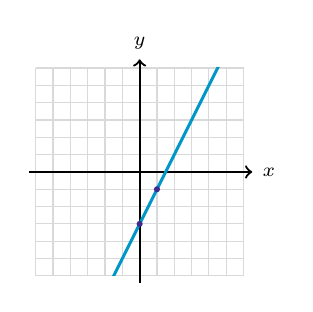
\begin{tikzpicture}[scale=0.22]
\draw[gray!30,thin] (-6,-6) grid (6,6);
\draw[->,thick] (-6.4,0)--(6.5,0) node[right,font=\scriptsize]{$x$};
\draw[->,thick] (0,-6.4)--(0,6.5) node[above,font=\scriptsize]{$y$};
\begin{scope}\clip (-6,-6) rectangle (6,6);
\draw[fmkey,line width=1.1pt] (-7,-17.000)--(7,11.000);
\end{scope}
\fill[fmtitle] (0.0,-3.0) circle (5pt);
\fill[fmtitle] (1.0,-1.0) circle (5pt);
\end{tikzpicture}\end{minipage}\end{tcolorbox}
\needspace{5.2cm}\par\vspace{2mm}\begin{tcolorbox}[enhanced,colback=white,colframe=fmwatch!60,boxrule=0.6pt,arc=1.5mm,left=3mm,top=1.5mm,bottom=1.5mm]\begin{minipage}[c]{0.58\linewidth}{\color{fmwatch}\bfseries 24.}\quad\small Plot $(0, 4)$, then use the slope $-\dfrac{1}{2}$: down 1, right 2.\par\vspace{1mm}\normalsize\textbf{Answer: $y = -\dfrac{1}{2}x + 4$}\end{minipage}\hfill\begin{minipage}[c]{0.38\linewidth}\centering 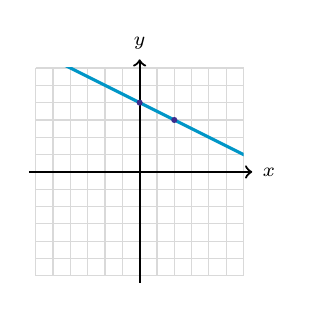
\begin{tikzpicture}[scale=0.22]
\draw[gray!30,thin] (-6,-6) grid (6,6);
\draw[->,thick] (-6.4,0)--(6.5,0) node[right,font=\scriptsize]{$x$};
\draw[->,thick] (0,-6.4)--(0,6.5) node[above,font=\scriptsize]{$y$};
\begin{scope}\clip (-6,-6) rectangle (6,6);
\draw[fmkey,line width=1.1pt] (-7,7.500)--(7,0.500);
\end{scope}
\fill[fmtitle] (0.0,4.0) circle (5pt);
\fill[fmtitle] (2.0,3.0) circle (5pt);
\end{tikzpicture}\end{minipage}\end{tcolorbox}
\needspace{5.2cm}\par\vspace{2mm}\begin{tcolorbox}[enhanced,colback=white,colframe=fmwatch!60,boxrule=0.6pt,arc=1.5mm,left=3mm,top=1.5mm,bottom=1.5mm]\begin{minipage}[c]{0.58\linewidth}{\color{fmwatch}\bfseries 25.}\quad\small Plot $(0, -1)$, then use the slope $\dfrac{2}{3}$: up 2, right 3.\par\vspace{1mm}\normalsize\textbf{Answer: $y = \dfrac{2}{3}x - 1$}\end{minipage}\hfill\begin{minipage}[c]{0.38\linewidth}\centering 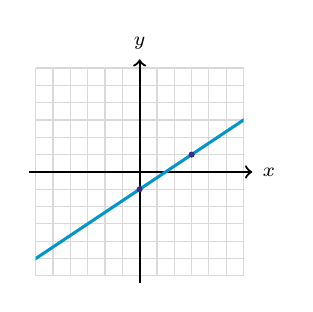
\begin{tikzpicture}[scale=0.22]
\draw[gray!30,thin] (-6,-6) grid (6,6);
\draw[->,thick] (-6.4,0)--(6.5,0) node[right,font=\scriptsize]{$x$};
\draw[->,thick] (0,-6.4)--(0,6.5) node[above,font=\scriptsize]{$y$};
\begin{scope}\clip (-6,-6) rectangle (6,6);
\draw[fmkey,line width=1.1pt] (-7,-5.667)--(7,3.667);
\end{scope}
\fill[fmtitle] (0.0,-1.0) circle (5pt);
\fill[fmtitle] (3.0,1.0) circle (5pt);
\end{tikzpicture}\end{minipage}\end{tcolorbox}
\needspace{5.2cm}\par\vspace{2mm}\begin{tcolorbox}[enhanced,colback=white,colframe=fmwatch!60,boxrule=0.6pt,arc=1.5mm,left=3mm,top=1.5mm,bottom=1.5mm]\begin{minipage}[c]{0.58\linewidth}{\color{fmwatch}\bfseries 26.}\quad\small Plot $(0, 2)$, then use the slope $-3$: down 3, right 1.\par\vspace{1mm}\normalsize\textbf{Answer: $y = -3x + 2$}\end{minipage}\hfill\begin{minipage}[c]{0.38\linewidth}\centering 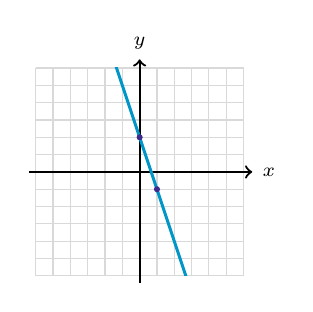
\begin{tikzpicture}[scale=0.22]
\draw[gray!30,thin] (-6,-6) grid (6,6);
\draw[->,thick] (-6.4,0)--(6.5,0) node[right,font=\scriptsize]{$x$};
\draw[->,thick] (0,-6.4)--(0,6.5) node[above,font=\scriptsize]{$y$};
\begin{scope}\clip (-6,-6) rectangle (6,6);
\draw[fmkey,line width=1.1pt] (-7,23.000)--(7,-19.000);
\end{scope}
\fill[fmtitle] (0.0,2.0) circle (5pt);
\fill[fmtitle] (1.0,-1.0) circle (5pt);
\end{tikzpicture}\end{minipage}\end{tcolorbox}
\needspace{4cm}\topicbar{Type 6 \quad Linear Functions in Real Life}
\keyitem{27}{$C = 2x + 3$; \ $2 \cdot 12 + 3 = 27$}{$C = 2x + 3$, \ \$27}
\keyitem{28}{$h = 30 - 2t$; \ $0 = 30 - 2t$ gives $t = 15$}{$h = -2t + 30$, \ 15 hours}
\keyitem{29}{$h = 1.5w + 4$; \ $1.5 \cdot 6 + 4 = 13$}{$h = 1.5w + 4$, \ 13 in}
\keyitem{30}{Start \$200 ($b$); loses \$15 each week ($m = -15$).}{$M = -15w + 200$; slope: $-\$15$ per week; intercept: \$200 at the start}
\end{document}
